\documentclass[]{article}
\usepackage{graphicx}
\usepackage[svgnames]{xcolor} 
\usepackage{fancyhdr}
\usepackage{tocloft}
\usepackage[hidelinks]{hyperref}
\usepackage{enumitem}
\usepackage[many]{tcolorbox}
\usepackage{listings }
%\usepackage[a4paper, total={6in, 8in} , top = 2cm,bottom = 4cm]{geometry}
\usepackage[a4paper, total={6in, 8in}]{geometry}
\usepackage{afterpage}
\usepackage{amssymb}
\usepackage{pdflscape}
\usepackage{textcomp}
\usepackage{xecolor}
\usepackage{rotating}
\usepackage[Kashida]{xepersian}
\usepackage[T1]{fontenc}
\usepackage{tikz}
\usepackage[utf8]{inputenc}
\usepackage{PTSerif} 
\usepackage{seqsplit}
\usepackage{changepage}


\usepackage{listings}
\usepackage{xcolor}
\usepackage{sectsty}

\setcounter{secnumdepth}{0}
 
\definecolor{codegreen}{rgb}{0,0.6,0}
\definecolor{codegray}{rgb}{0.5,0.5,0.5}
\definecolor{codepurple}{rgb}{0.58,0,0.82}
\definecolor{backcolour}{rgb}{0.95,0.95,0.92}
\definecolor{blanchedalmond}{rgb}{1.0, 0.92, 0.8}
\definecolor{brilliantlavender}{rgb}{0.96, 0.73, 1.0}
 
\NewDocumentCommand{\codeword}{v}{
\texttt{\textcolor{blue}{#1}}
}
\lstset{language=java,keywordstyle={\bfseries \color{blue}}}

\lstdefinestyle{mystyle}{
    backgroundcolor=\color{backcolour},   
    commentstyle=\color{codegreen},
    keywordstyle=\color{magenta},
    numberstyle=\tiny\color{codegray},
    stringstyle=\color{codepurple},
    basicstyle=\ttfamily\normalsize,
    breakatwhitespace=false,         
    breaklines=true,                 
    captionpos=b,                    
    keepspaces=true,                 
    numbers=left,                    
    numbersep=5pt,                  
    showspaces=false,                
    showstringspaces=false,
    showtabs=false,                  
    tabsize=2
}

\lstset{style=mystyle}

 \settextfont[BoldFont={XB Zar bold.ttf}]{XB Zar.ttf}


\setlatintextfont[Scale=1.0,
 BoldFont={LiberationSerif-Bold.ttf}, 
 ItalicFont={LiberationSerif-Italic.ttf}]{LiberationSerif-Regular.ttf}




\newcommand{\inputsample}[1]{
    ~\\
    \textbf{ورودی نمونه}
    ~\\
    \begin{tcolorbox}[breakable,boxrule=0pt]
        \begin{latin}
            \large{
                #1
            }
        \end{latin}
    \end{tcolorbox}
}

\newcommand{\outputsample}[1]{
    ~\\
    \textbf{خروجی نمونه}

    \begin{tcolorbox}[breakable,boxrule=0pt]
        \begin{latin}
            \large{
                #1
            }
        \end{latin}
    \end{tcolorbox}
}

\newtcolorbox{mybox}[2][]{colback=red!5!white,
colframe=red!75!black,fonttitle=\bfseries,
colbacktitle=red!85!black,enhanced,
attach boxed title to top center={yshift=-2mm},
title=#2,#1}

\newenvironment{changemargin}[2]{%
\begin{list}{}{%
\setlength{\topsep}{0pt}%
\setlength{\leftmargin}{#1}%
\setlength{\rightmargin}{#2}%
\setlength{\listparindent}{\parindent}%
\setlength{\itemindent}{\parindent}%
\setlength{\parsep}{\parskip}%
}%
\item[]}{\end{list}}


\definecolor{foldercolor}{RGB}{124,166,198}
\definecolor{sectionColor}{HTML}{ff5e0e}
\definecolor{subsectionColor}{HTML}{008575}

\definecolor{listColor}{HTML}{00d3b9}

\definecolor{umlrelcolor}{HTML}{3c78d8}

\definecolor{subsubsectionColor}{HTML}{3c78d8}

\defpersianfont\authorFont[Scale=0.9]{XB Zar bold.ttf}

\defpersianfont\titr[Scale=1.5]{Lalezar-Regular.ttf}

\defpersianfont\fehrest[Scale=1.2]{Lalezar-Regular.ttf}

\defpersianfont\fehrestTitle[Scale=3.0]{Lalezar-Regular.ttf}

\defpersianfont\fehrestContent[Scale=1.2]{XB Zar bold.ttf}


\sectionfont{\color{sectionColor}}  % sets colour of sections
\subsectionfont{\color{subsectionColor}}  % sets colour of sections
\subsubsectionfont{\color{subsubsectionColor}}


\renewcommand{\labelitemii}{$\circ$}


\renewcommand{\baselinestretch}{1.1}


\renewcommand{\contentsname}{فهرست}

\renewcommand{\cfttoctitlefont}{\fehrestTitle}


\renewcommand\cftsecfont{\color{sectionColor}\fehrestContent\selectfont}
\renewcommand\cftsubsecfont{\color{subsectionColor}\fehrestContent\selectfont}
\renewcommand\cftsubsubsecfont{\color{subsubsectionColor}\fehrestContent\selectfont}
%\renewcommand{\cftsecpagefont}{\color{sectionColor}}

\setlength{\parskip}{1.2pt}

\begin{document}


%%% title pages
\begin{titlepage}
\begin{center}

\textbf{ \Huge{به نام خدا} }
        
\vspace{0.2cm}


\includegraphics[width=0.4\textwidth]{sharif1.png}\\
\vspace{0.2cm}
\textbf{ \Huge{\emph درس برنامه‌سازی پیشرفته} }\\
\vspace{0.25cm}
\textbf{ \Large{امنیت شبکه} }
\vspace{0.2cm}
       
 
      \large \textbf{دانشکده مهندسی کامپیوتر}\\\vspace{0.1cm}
    \large   دانشگاه صنعتی شریف\\\vspace{0.2cm}
       \large   ﻧﯿﻢ سال دوم 99-98 \\\vspace{0.10cm}
      \noindent\rule[1ex]{\linewidth}{1pt}
اساتید:\\
    \textbf{{مهدی مصطفی‌زاده، ایمان عیسی‌زاده، امیر ملک‌زاده، علی چکاه}}



        \vspace{0.10cm}
نگارش و تهیه محتوا:\\
    \textbf{{محسن دهقان کار، صابر ظفرپور}}
    
       \vspace{0.10cm}
       تنظیم داک:\\
    \textbf{{امیرمهدی نامجو، محسن دهقان کار}}

    
        \vspace{0.05cm}
    

\end{center}
\end{titlepage}
%%% title pages


%%% header of pages
\newpage
\pagestyle{fancy}
\fancyhf{}
\fancyfoot{}
\cfoot{\thepage}
\lhead{امنیت شبکه}
\rhead{
\includegraphics[width=0.1\textwidth]{sharif.png}\\
دانشکده مهندسی کامپیوتر
}
\chead{پروژه برنامه‌سازی پیشرفته}
%%% header of pages
\renewcommand{\headrulewidth}{2pt}

\KashidaOff



\tableofcontents

\newpage

 \Large \textbf{\\\\
}


\section*{{\titr امنیت یعنی چی؟}}
\addcontentsline{toc}{section}{{\fehrestContent امنیت یعنی چی؟}}

به طور کلی همه ی ما یک ذهنیت اولیه (احتمالا اشتباه) از امنیت داریم، در این داک ما قصد داریم یک توضیح مختصر و البته پوشا از موضوعات مرتبط با امنیت در فاز 3 پروژه این ترم AP به شما عزیزان ارائه دهیم. امنیت در کامپیوتر یا به عبارت دیگر همان امنیت سایبری یکی از شاخه‌های مهم حوزه کامپیوتر است که در عصر ارتباطات و با افزایش تصاعدی ضریب نفوذ کامپیوتر در عرصه‌های مختلف نیاز به آن نیز در حال افزایش است. در دانشکده ما نیز این درس جزو چارت اجباری (ترم 8) است.


\section*{{\titr شاخه‌های مختلف امنیت}}
\addcontentsline{toc}{section}{{\fehrestContent شاخه‌های مختلف امنیت}}
در این داک ما تنها قصد داریم که امنیت را در سطوح شبکه به صورت محدود بررسی کنیم و در این سطح نیز فقط به موضوعات امنیت نرم افزار در سطح شبکه کفایت می‌کنیم. از دیگر شاخه‌های مهم بحث سایبر سکیوریتی \lr{(cyber security)} می‌توان به امنیت در حوزه اینترنت اشیا، امنیت زیرساخت‌های سخت افزاری، امنیت در چرخه تولید و حیات نرم افزار و … اشاره کرد.




\section*{{\titr تهدیدات و آسیب پذیری ها و کنترل ها}}
\addcontentsline{toc}{section}{{\fehrestContent تهدیدات و آسیب پذیری ها و کنترل ها}}
در مبحث امنیت ما با تهدیداتی روبرو هستیم، اما ابتدا باید تهدید را به طور دقیق تعریف کنیم:


تهدید(Threat): یک خطر بالقوه که می‌تواند از یک آسیب پذیری موجود درون سیستم سوء استفاده کند.

به طور مثال: درز اطلاعات بانکی حساب‌های درون فروشگاه شما  - آسیب‌های فیزیکی به سرور‌های فروشگاه شما نظیر سیل و زلزله و حریق 

اما در تعریف تهدید به کلمه آسیب پذیری برخوردیم ، پس باید برای آن نیز یک تعریف دقیق ارائه   کنیم:


\bigskip
آسیب پذیری(Vulnerability) : ضعفی که درون سیستم وجود دارد و می‌تواند توسط یک عامل (به طور مثال یک هکر) برای رسیدن به اهداف (معمولا خصمانه) استفاده شود.

به طور مثال: آسیب پذیری  \href{https://owasp.org/www-community/attacks/xss/}{\textcolor{blue}{\underline{\lr{\lr{(Cross Site Scripting XSS)}}}}}  - آسیب پذیری عدم رمزگذاری ارتباط کلاینت و سرور و …

برای مقابله با این آسیب پذیری‌ها می‌توان یک سری راهکار امنیتی پیشنهاد کرد که با اجرای آن می‌توان بسیاری از آسیب پذیری‌های شناخته شده را برطرف کرد.

به طور مثال :\lr{(Input Sanitization)}  یک کنترل بسیار قوی برای جلوگیری از حملات تزریق است. 

\bigskip

در ادامه سعی می‌کنیم بسیاری از آسیب پذیری‌هایی که ممکن است در نرم افزار شما وجود داشته باشد را به شما اطلاع داده و راهکار و ابزار‌های شناسایی آن و راهکار مناسب برطرف کردن آن و کنترل‌های مناسب برای آن آسیب پذیری را در زبان جاوا در اختیارتان قرار دهیم.

\newpage

\section*{{\titr آسیب پذیری ها و حملات رایج}}
\addcontentsline{toc}{section}{{\fehrestContent آسیب پذیری ها و حملات رایج}}

\lr{
\begin{enumerate}
\item
Replay attacks*
\item
Improper Inputs*
\item
Sql Injection* (When using SQL-Based database)
\item
Broken Authentication*
\item
Sensitive Data Exposure
\item
Brute force attack*
\item
Broken Access Control
\item
Remote Code Execution (RCE)
\item
Man In The Middle (MITM)
\item
Denial of service* (DOS)
\end{enumerate}
}


جزییات این آسیب پذیری‌ها در ادامه قرار داده شده است.




\section*{{\titr خب من کجا می‌تونم این حملاتو تست کنم و قلقشونو بگیرم؟؟}} 

بسیار سوال خوبیه، شما هر چقدر هم در مورد این آسیب پذیری‌ها مطالعه کنید ، در صورتی که این آسیب پذیری‌ها توسط خودتون تست نشه و به نوعی خودتون در جایگاه فرد هکر نباشید، نخواهید توانست که به خوبی نسبت به امنیت نرم افزار خودتون دید خوبی داشته باشید. اما تست کردن این حملات بر روی سایت‌های واقعی میتونه براتون عواقب بدی داشته باشه:)

خب برای این موضوع بهترین راهکار تست کردن این باگ‌ها درون یک محیط ایزوله آزمایشگاهی هست، پس هر وقت که حوصله داشتید برید توی این سایت و نرم افزار \href{https://webgoat.github.io/WebGoat/}{\textcolor{blue} {webgoat}}  رو نصب کنید و یک تجربه جذابی از هکر بودن (حداقل توی آزمایشگاه) رو داشته باشید.



\section*{{\titr جزییات آسیب پذیری‌ها}}
\addcontentsline{toc}{section}{{\fehrestContent جزییات آسیب پذیری‌ها}}


\subsection*{{\lr{\titr Replay Attacks}}}
\addcontentsline{toc}{subsection}{{\fehrestContent Attacks Replay}}
همان طور که اسمش پیداست، این حمله زمانی رخ می‌دهد که یک مهاجم (\lr{‌attacker}) پیام‌های رد و بدل شده بین سرور و کلاینت شما را برای خود ذخیره می‌کند(\lr{intercepting and capturing packets})، سپس پس از مدتی آن‌ها را دوباره به مقصد می‌فرستد یا حجم زیادی از این پیام‌ها را از طرف خودش به مقصد می‌فرستد. حال اگر دریافت کننده پیام، با این پیام‌های تکراری کاری انجام دهد که مطلوب نیست، \lr{replay attack} رخ داده است.

برای توضیحات بیش‌تر به این \href{https://www.kaspersky.com/resource-center/definitions/replay-attack} {\textcolor{blue}{\underline{لینک}}} مراجعه کنید.




\subsection*{{\lr{\titr Improper Inputs}}}
\addcontentsline{toc}{subsection}{{\fehrestContent Inputs Improper}}
ممکن است به سمت سرور شما هر نوع ورودی فرستاده شود. اگر در سمت سرور (گیرنده پیام) هیچ اعتبار سنجی (validation)‌ و یا اعتبار سنجی ضعیفی انجام شود،‌ ممکن است سبب متوقف شدن سرور  مثلا پرتاب شدن exception و یا تغییر در وضعیت سرور شود که مطلوب نیست. هدف این حمله این است که با دادن ورودی‌های نامعتبر به سرور دچار خلل در کار سرور شویم. یا به عبارتی دسترسی پذیری (‌availability)‌ سرور را از بین ببرد.
\bigskip

همچنین حالت‌هایی را درنظر بگیرید که کلاینت و سرور پیامی را با هم رد و بدل کردند،‌ شخصی در این بین این پیام را شنود کرد (‌کاری که در شبکه انجام دادنش اصلا سخت نیست برای مثال با استفاده از برنامه ای مثل wireshark). سپس این فرد شنودکننده،‌ پیام را تغییر می‌دهد و برای سرور مجددا می فرستد. نباید با این کار اثر نامطلوبی بر روی عملکرد سرور ایجاد شود.

\bigskip

حالتی دیگر این است که سرور به کلاینت این اجازه را بدهد که نامی با هر طولی وارد کند، بنابراین کلاینت (فرستنده)‌ می‌تواند با نوشتن یک رشته بسیار طولانی، حجم بزرگی از حافظه سرور را اشغال کند و با تکرار این عمل،‌ سرور را کُند کرده و یا از کار بیندازد.

این یک آسیب پذیری کلی، ابتدایی و در عین حال خطرناک است،‌ برای مطالعه بیشتر در مورد آن به این \href{https://cwe.mitre.org/data/definitions/20.html}{\textcolor{blue}{\underline{{لینک}}}} مراجعه کنید.




\subsection*{{\lr{\titr SQL-Injection}}}
\addcontentsline{toc}{subsection}{{\fehrestContent SQL-Injection}}
در صورت استفاده از دیتابیس‌های SQL ، این حملات می تواند کاملا دیتابیس شما را پاک کند یا اینکه در آن تغییرات مورد‌نیاز نفوذگر را پیاده کند، از این حملات برای دور زدن صفحات احراز هویت نیز استفاده می‌شود. اما در زبان جاوا راهکار‌ها و کنترل‌های بسیار کارایی برای مقابله با این حملات وجود دارد که شما باید در هنگام نوشتن نرم افزار خود از آن استفاده کنید.

این \href {"https://software-security.sans.org/developer-how-to/fix-sql-injection-in-java-using-prepared-callable-statement"}{\textcolor{blue}{\underline{لینک}}} 
راهکار عملی رفع این آسیب پذیری را در زبان جاوا نشان می‌دهد. اما پیش از آن بهتر است در مورد این آسیب پذیری \href {https://www.w3schools.com/sql/sql_injection.asp}{\textcolor{blue}{\underline{مطالعه}}} داشته باشد.



\subsection*{{\lr{\titr Broken Authentication}}}
\addcontentsline{toc}{subsection}{{\fehrestContent Authentication Broken}}
هدف اولیه و اصلی حمله کننده (attacker) به سرور، این است که بدون داشتن اطلاعات صحیح (مثلا یوزر و پسورد)، خودش را به جای شخص دیگری جا بزند یا به عبارتی وانمود کند که شخص دیگری است. برای این دسته از کارها او باید احراز هویت سرور (authentication)‌را دور بزند. برای این کار می‌تواند از روش‌های مختلفی استفاده کند یا در واقع احراز هویت شما ممکن است به اشکال مختلفی فریب بخورد.

اشکال مختلف این حمله و همچنین راه‌های جلوگیری از آن‌ها در این \href{https://hdivsecurity.com/owasp-broken-authentication}{\textcolor{blue}{\underline{لینک}}} قابل مشاهده است.




\subsection*{{\lr{\titr Sensitive Data Exposure}}}
\addcontentsline{toc}{subsection}{{\fehrestContent Exposure Data Sensitive}}
برنامه شما اطلاعاتی از کاربران مختلف دارد. این اطلاعات همواره باید محرمانه باقی بمانند.(confidentiality) مثلا در این پروژه، یک خریدار عادی نباید بتواند اطلاعات کاربری مدیر فروشگاه را بفهمد. یا بعنوان مثال دیگر وقتی خریدار وارد اکانت خود می‌شود،‌ نباید اطلاعات مربوط به یوزر و پسورد و یا هرنوع اطلاعات دیگری از او، توسط شخصی که صرفا پیام‌های رد و بدل شده را شنود می‌کند، قابل دیدن و شناسایی باشد. 

مثلا به‌عنوان مثال برای اینکه پیام‌های رد و بدل شده شنود نشوند می‌توان از رمزنگاری استفاده کرد. رمزنگاری از رایج‌ترین کنترل‌ها برای حفظ محرمانگی پیام‌های در حال انتقال و همچنین پیام‌های ذخیره شده در حافظه است.

\subsection*{{\lr{\titr Brute force attack}}}
\addcontentsline{toc}{subsection}{{\fehrestContent Attack force Brute}}
در صورتی که کاربری قصد داشته باشد برای دور زدن یک فرم در نرم افزار شما (به طور مثال یک فرم ورود به حساب کاربری) تعداد زیادی تلاش ناموفق می‌کند و سعی می‌کند با حدس زدن، ورودی درست را پیدا کند. این کار می‌تواند هم به مانند آسیب پذیری DoS عمل کند و هم می‌تواند باعث به مخاطره افتادن اطلاعات حیاتی نظیر رمز کاربران شود.

\bigskip

ساده‌ترین روش کنترل قرار دادن یک شمارنده برای تعداد تلاش‌های ناموفق هر IP است ، به طور مثال اگر یک IP در کمتر از 10 ثانیه بیش از 5 (با توجه به نوع برنامه و سرویس شما این عدد متفاوت است) درخواست اشتباه برای سرور فرستاد، باید آن IP توسط سرور در لیست سیاه موقت قرار گیرد و اجازه اتصال به آن به صورت موفق داده نشود.

\subsection*{{\lr{\titr Broken Access Control}}}
\addcontentsline{toc}{subsection}{{\fehrestContent Control Access Broken}}
کنترل دسترسی یا \lr{access control} بخشی از سیستم است که مشخص می‌کند چه کسی چه اجازه‌ای دارد. مثلا در این پروژه، مدیر فروشگاه یکسری دسترسی‌هایی دارد که خریدار عادی ندارد. این دسترسی‌ها باید کنترل شوند. 
\bigskip
مثلا در سیستم عامل شما، ممکن است کاربران (user)‌ متفاوتی وجود داشته باشند و یک کاربر به فایل‌های کاربر دیگر دسترسی نداشته باشه و یا مثلا فقط اجازه خواندن از آن‌ها را داشته باشد (و نه نوشتن). کنترل کردن و هندل کردن این دسترسی‌ها و اجازه دادن به یک شخص (‌subject‌) که از یک منبع (‌object‌) استفاده کند،‌ توسط \lr{access control} انجام‌می شود. 

حال اگر بتوان به راحتی کنترل دسترسی را دور زد و مثلا یک خریدار بتواند خودش را به جای مدیر فروشگاه جا بزند، این یک آسیب پذیری محسوب می‌شود و امنیت را نقض می‌کند.


\subsection*{{\lr{\titr Remote Code Execution}}}
\addcontentsline{toc}{subsection}{{\fehrestContent Execution Code Remote}}
از جمله آسیب پذیری‌های یک سیستم (‌بطور خاص یک سرور)، این است که کلاینت (هر کسی که به‌عنوان کاربر برای آن سرور محسوب می‌شود) بتواند کدی مخرب را بر روی آن بفرستد و اجرا کند. نام دیگر آن \lr{code injection} نیز هست.



به این کار exploit کردن نیز گفته می‌شود و روش‌های بسیار متنوعی دارد. برای مطالعه بیشتر به این \href{https://owasp.org/www-community/attacks/Code_Injection}{\textcolor{blue}{\underline{لینک}}}  مراجعه کنید. البته این حمله و فهمیدن مثال‌‌های آن نیاز به یکسری پیش زمینه‌هایی دارد که بهترین کار برای افراد علاقه مند جست و جو کردن و رفتن به سمت این مباحث است. 



\subsection*{{\lr{\titr Man In The Middle}}}
\addcontentsline{toc}{subsection}{{\fehrestContent Middle The In Man}}
این حمله، حمله بسیار معروفی است که متوجه بسیاری از ارتباطات (‌communication) است. مثل فرض کنید محسن۱ و محسن۲  می‌خواهند از طریق شبکه با هم صحبت کنند (شبکه را صرفا یک سری کابل در نظر بگیرید که پیام را از یک فرد گرفته و به دیگری می‌رساند). همچنین فرض کنید در این شبکه (یه مشت کابل)‌ یک نفر سومی به اسم صابر، یک کابل را قطع می‌‌کند و خودش بین این دو سرِ کابل می‌نشیند.

\bigskip

حال محسن۱ می‌خواهد به محسن۲ سلام بگوید. محسن۱ پیام را روی کابل می‌فرستد (نزدیکترین کابل به خودش) و این پیام به راهش ادامه می‌دهد تا این که به کابل قطع شده (صابر)‌می‌رسد، صابر که آدم ناجوری است(!!) این پیام را از یک سرِ کابل قطع شده گرفته، آن را به یک فحش تبدیل می‌کند و آن پیام را برروی آن یکی سرِ کابل قطع شده به سمت محسن۲ می‌فرستد.

همان طور که دیدید، در واقع صابر پیام خودش را به جای پیام محسن۱ به محسن۲ می‌رساند و بالعکس.

\bigskip
این حمله در تصویر زیر نیز نشان داده شده است و مسلما خطرات زیادی دارد.

\begin{figure}
  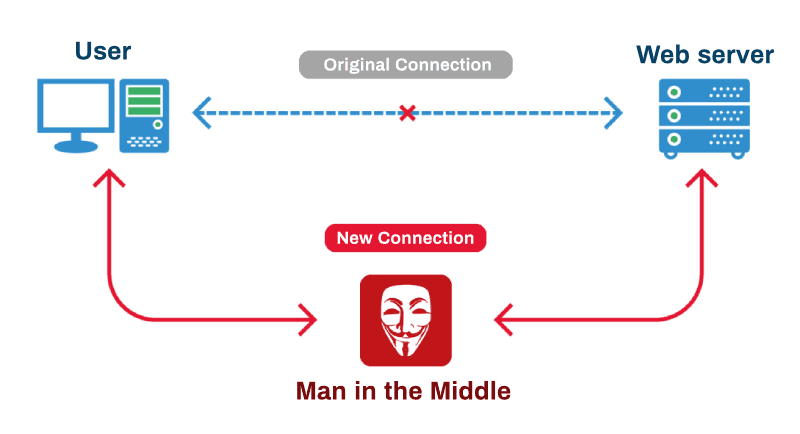
\includegraphics[width=\linewidth]{images/man-in-the-middle.png}
\end{figure}
\bigskip

برای مطالعه بیش‌تر و دقیق‌تر در مورد این نوع حمله به این \href{https://www.imperva.com/learn/application-security/man-in-the-middle-attack-mitm/}{\textcolor{blue}{\underline{لینک}}}
 و این \href{https://en.wikipedia.org/wiki/Man-in-the-middle_attack}{\textcolor{blue}{\underline{لینک}}} مراجعه کنید.





\subsection*{{\lr{\titr Denial of Service (DoS)}}}
طبیعی است که هر نرم افزاری با کاربر خود در ارتباط است و تعدادی پیام با سرور جابجا می‌شود، اما گاهی فرد خرابکار سعی می‌کند با استفاده از یک کد تعداد بسیار زیادی درخواست به سرور شما در مدت زمان کم ارسال کند و با توجه به محدود بودن نرخ پذیرش پیام توسط سرور‌، باعث مختل شدن کل سرور و از کار افتادن سرویس شما می‌شود، پس شما باید با روش‌های هوشمندانه جلوی این رفتارهای خرابکارانه را بگیرید.
\bigskip

ساده ترین روش کنترل قرار دادن یک شمارنده برای هر IP است ، به طور مثال اگر یک IP در کمتر از 10 ثانیه بیش از 100 (با توجه به نوع برنامه و سرویس شما این عدد متفاوت است) درخواست برای سرور فرستاد، باید آن IP توسط سرور در لیست سیاه قرار گیرد و اجازه اتصال به آن داده نشود. (در صورتی که فرد خرابکار از تعداد زیادی IP برای حمله به سرویس شما استفاده کند این راهکار شکست می‌خورد، به آن نوع از حملات انکار، \lr{Distributed Denial of Service} یا DDoS می‌گویند.)

\section*{{\titr پس پروژه چی شد این وسط؟؟}}
\addcontentsline{toc}{section}{{\fehrestContent پس پروژه چی شد این وسط؟؟}}
آسیب پذیری‌هایی که می‌توانید در پروژه‌تان جلویش را بگیرید و برای نمره‌ی امتیازی چک می‌شوند (در واقع چک کردنشون سخت نیست!‌)، فقط موارد ستاره دار در لیست بالا هستند. (‌البته ممکن است موارد دیگری هم در داک مربوط به امتیازات اضافه شود.)

\begin{itemize}
\item
برای بررسی کردن و نمره دادن به این بخش، از شما یک \textcolor{red}{مستند} (یا در کل یک گزارش مکتوب) از کارهایی که برای رفع این آسیب پذیری‌ها و حملات انجام دادید، خواسته می‌‌شود. این که مستند چطور نوشته شود خیلی اهمیت ندارد اما باید هر کاری که برای جلوگیری از حمله مد نظر انجام دادید را قید کنید و مواردی که نوشته باشید، چک خواهند شد.
\item
همچنین نیازی نیست جلوی همه‌ی حملات ستاره دار را بگیرید‌،‌ هر حمله نمره خاص خود را خواهد داشت.
\end{itemize}


\section*{{\titr سایر منابع}}
\addcontentsline{toc}{section}{{\fehrestContent سایر منابع}}

برای مشاهده آخرین آسیب پذیری‌های ثبت شده، هرگونه اطلاعات آماری و آسیب پذیری‌های مربوط به یک محصول یا شرکت خاص دیتابیس‌هایی موجود هستند و این آسیب پذیری‌ها را ثبت می‌کنند و به آن‌ها شناسنامه می‌دهند. از جمله معروف‌ترین‌ها CVE است.

\begin{flushleft}
\url {https://www.cvedetails.com}
\end{flushleft}
\bigskip

همچنین بنیادی تحت عنوان \lr{Open Web Application Security Project}  یا OWASP با هدف بهبود امنیت نرم افزار وجود دارد و مثلا پروژه‌ای تحت عنوان \lr{OWASP Top 10 Web Application Security Risks} وجود دارد که هر ساله لیستی از رایج‌ترین ریسک‌ها در زمینه برنامه‌های تحت وب ارائه می‌دهد. ( و بطور مشابه پروژه‌ای برای موبایل و … )

\begin{flushleft}
\url{https://owasp.org/www-project-top-ten}
\end{flushleft}

\bigskip
هم چنین مسابقاتی تحت عنوان CTF یا  \lr{Capture The Flag} برگزار می‌شوند که چالش‌هایی برای شرکت کنندگان دارند. خوب است در این زمینه هم جست و جویی داشته باشید. این رویداد امسال از طرف دانشکده خودمان هم انجام شد:

\begin{flushleft}
\url{https://susec.tf}
\end{flushleft}





\newpage



\end{document}







